\documentclass[a4paper, 11pt]{article}

\usepackage[utf8]{inputenc} %if your LaTeX editor does not support
% Unicode (UTF8),
% change this option to ansinew or latin1 if you need additional
% packages, load them here, but mind possible interference with the
% DokDok package!
\usepackage{courier}
\usepackage{dokdok}
%\usepackage{refcheck}
\usepackage{units}
\usepackage{color}

\begin{document}

\dokdoktitle{Spatio-angular microscopy}

\dokdokauthor{Martin Kielhorn\sup{*1,2}, and Rainer
  Heintzmann\sup{1,2,3}}

\dokdokaffiliation{ \sup{1}Institute of Photonic Technology,
  Albert-Einstein Str. 9, 07745 Jena, Germany}

\dokdokaffiliation{ \sup{2}Randall Division of Cell \& Molecular
  Biophysics, King's College London, NHH, Guy's Campus, London SE1
  1UL, U.K.}

\dokdokaffiliation{ \sup{3}Institute of Physical Chemistry,
  Friedrich-Schiller-Universität Jena, Helmholtzweg 4, 07743 Jena,
  Germany}

\dokdokemail{kielhorn.martin@gmail.com}
\raggedbottom

\begin{abstract}
  \noindent \bfseries{ Photobleaching and phototoxicity pose a problem
    in live cell imaging. Excessive excitation light can induce
    reactive oxygen species in observed organisms. These can disturb
    signalling pathways and alter the natural response of the
    sample. We augment a widefield epifluorescence microscope with two
    spatial light modulators (SLM). These allow illumination with
    arbitrary patterns. Depending on the distribution of fluorophores
    a considerable reduction in photobleaching and phototoxicity can
    be expected.}
\end{abstract}

\begin{multicols}{2}

\dokdoksection{Introduction}

In a fluorescence microscope excitation light is shone through an
objective onto a specimen containing fluorophores. These fluorophores
absorb excitation light and subsequently emit photons of lower
energy. The fluorescence light of in-focus fluorophores is formed into
a sharp image, light from out-of-focus areas deteriorates the image by
creating a blurred background.

 
Nowadays it is common to observe the dynamic properties of
fluorescently labelled proteins and extract quantitative information
about the structures they form within living cells. The length of the
study and the accuracy of the result of a given experiment, however,
is limited by photobleaching and light induced toxicity in the
biological specimen.

One of the by-products of fluorophore excitation is reactive singlet
oxygen. The oxidative stress can lead to cell death or more subtle
effects such as the suppression of normal cell signalling functions.

In order to extend experiments in time and to follow the fate of cells
over many generations, a substantial reduction illumination would be
desired.

In ultra microscopy a thin sheet of excitation light is sent from the
side along the focal plane of a widefield microscope. Its results are
impressive \cite{Huisken2004}. However, mounting the samples is
difficult and long range objectives are used, which limit the
collection angles, detection efficiency and resolution.

In \cite{Hoebe2007} a variant of a confocal microscope is developed,
that illuminates the specimen according to local fluorophore
concentration. Dim areas are only illuminated until the fluorophore
content is confirmed to be below the threshold. Areas with high
fluorophore content are only illuminated until a certain photon count
is reached. Areas of intermediate brightness are illuminated for the
full time. The resulting image is of the same perceived image quality
as a conventional confocal image but at much lower dosage.

Temporal focusing (TF) and generalised phase contrast (GPC) have been
combined in \cite{Papagiakoumou2010}. For TF the ultra-short
excitation pulse is diffracted on a grating in an intermediate
image. The spectral components enter along a line on the pupil of the
objective and only excite fluorophores in a sheet around the focal
plane, where they arrive simultaneously. The GPC allows spatial
exposure control in the focal plane.

In \cite{Levoy2009} a micro-lens-based microscope for simultaneous
detection of angular and spatial information about the light returning
from the sample is shown. Applying their technique for illumination
would give a spatio-angular excitation microscope comparable to
ours. It would allow simultaneous exposure of in-focus areas with
different angles. However, the micro-lenses define the trade-off
between angular and spatial resolution. Our approach is more flexible
and better suited as a prototype to establish useful illumination
schemes.

\dokdoksection{Spatio-angular microscope} Figure \ref{fig:system}
shows a schematic of our microscope. A rotating micro-lens array and a
light tunnel provide uniform illumination in the plane $F'''$, which
is conjugate to the field $F$ in the specimen. SLM1 is an array of
$256\times 256$ torsional micro-mirrors. When the mirrors are tilted,
they act as a diffraction grating. The aperture $B_1$ only transmits
the zero order of the grating and the lens $L_2$ forms an intensity
image of SLM1 in $P'$.


\begin{figure}[H]
\centeringx
{\scriptsize \input{memi-real.pdf_tex}}
\caption{Schematic of our microscope. SLM = spatial light modulator,
  PBS = polarizing beam splitter, DBS = dichroitic beam splitter, TL =
  tube lens. %, B = circular aperture. % this doesn't fit1
}
\label{fig:system}
\end{figure}

A polarizing beam splitter illuminates SLM2. This display is based on
ferroelectric liquid crystals (FLC). The optic axis of the FLC in each
pixel can have two orientations, depending on the applied voltage. An
on-pixel acts as a $\lambda/4-$plate and rotates the returning light
by $90^\circ$. An off-pixel has no effect on the polarization.


 SLM1 is imaged into the back focal plane $P$ of the
objective. SLM2 is conjugate to the focal plane $F$ in sample space.
SLM1 controls the illumination angles while SLM2 selects the area in
the sample, that will be illuminated.


\paragraph{Experimental verification.}
The diagram in Figure \ref{fig:ray}~right, depicts a three-dimensional
distribution of beads with \unit[2]{$\mu$m} diameter. The data was
obtained by projecting gratings with SLM2 into the specimen and
reconstructing optically sectioned slices. After the positions of the
beads were known, they were selectively illuminated with SLM1 patterns
as shown in \ref{fig:ray}~left. These patterns were computed by
finding areas in the pupil that excite the target bead without
exposing out-of-focus beads.

\begin{figure}[H]
 \centering
 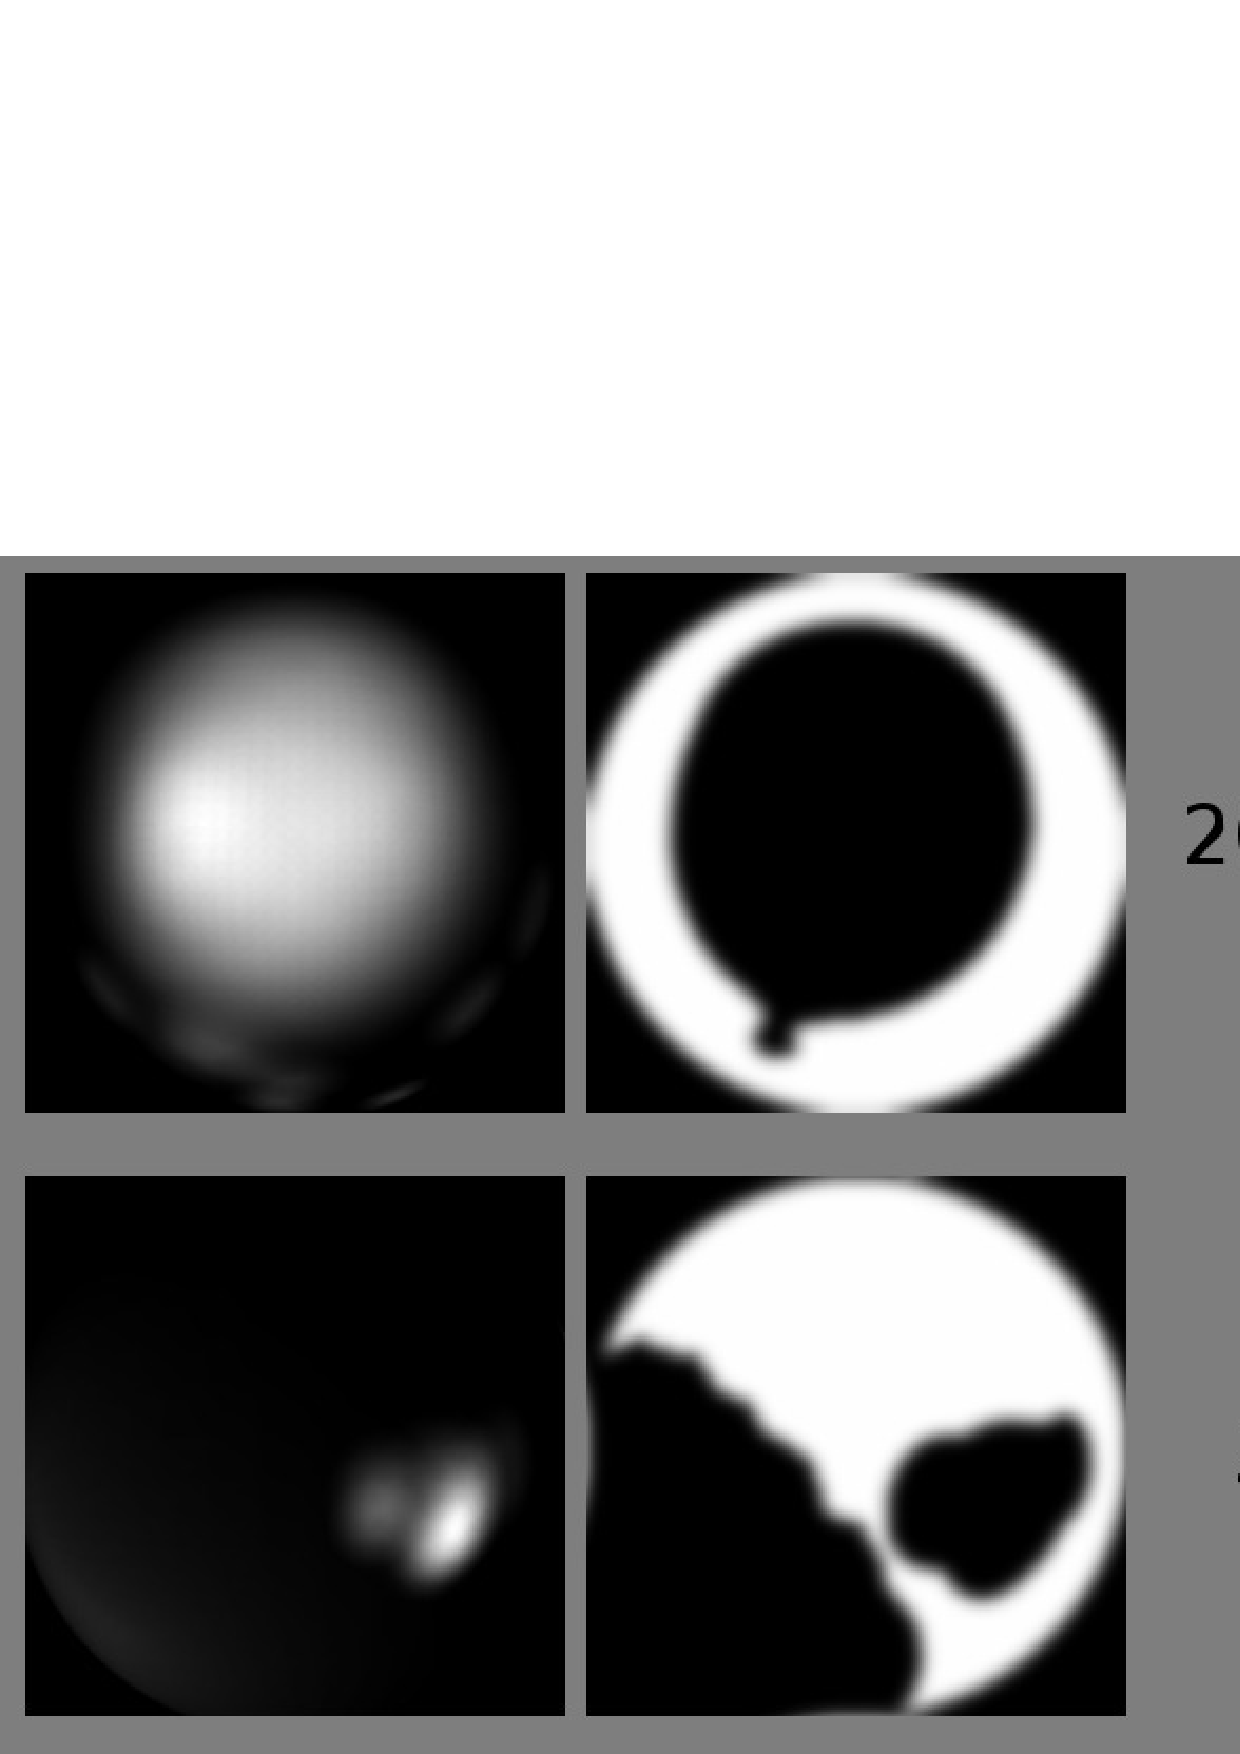
\includegraphics[width=0.48\textwidth]{bfp2-bfp-images-and-model}
\caption{{\bf right:} Sphere model of a
  sample with three-dimensionally distributed beads. {\bf left:}
  Optimized SLM1 masks to illuminate bead 26 or bead 5.}
\label{fig:ray}
\end{figure}


A similar approach can be used for time-laps imaging of nuclei in
developing embryos. Their structure doesn't change much from one time
frame to the next and one could predict the position of the nuclei
using the current image stack, while preparing the illumination
patterns for the acquisition of the next stack.


\dokdoksection{Conclusion} We built a microscope that can
simultaneously control the pattern of the excitation illumination in
the pupil $P$ of the objective and the front focal plane $F$ in the
specimen.

The two separate displays give the flexibility that is needed in order
to investigate illumination strategies while the Heisenberg
uncertainty principle prevents tight simultaneous control in the
Fourier planes $F$ and $P$.
\end{multicols}

\begin{center}
\rule{0.75\textwidth}{1pt}
\end{center}

\bibliographystyle{dokdok}
\bibliography{all}
\end{document} 


